\documentclass[10pt,leqno]{amsart}
\usepackage{graphicx}
\baselineskip=16pt
\usepackage{indentfirst,csquotes}

\topmargin= .5cm
\textheight= 20cm
\textwidth= 32cc
\baselineskip=16pt

\evensidemargin= .9cm
\oddsidemargin= .9cm

\usepackage{datetime}
\usepackage{wrapfig}
\usepackage{enumerate}
\usepackage{graphicx}
\usepackage{caption}
\usepackage{siunitx}
\usepackage{subcaption}
\usepackage{amsmath}
\usepackage{array,tabularx}
\usepackage{chngcntr}
\usepackage{afterpage}
\usepackage{ulem}
\usepackage{hyperref}
\usepackage{dirtytalk}
\usepackage{algorithm2e}
\usepackage{enumitem,amssymb}
\usepackage{pifont}
\usepackage{amsmath}
\usepackage{listings}
\usepackage{xcolor}
\usepackage{formal-grammar}
\usepackage{varwidth}
\usepackage{fmtcount}
\usepackage{tikz}
\usepackage{array}
\usepackage[framemethod=tikz]{mdframed} % Allows defining custom boxed/framed environments
\usepackage{cleveref}
\usepackage{microtype}
\usepackage{dirtytalk}

\usetikzlibrary{trees}
\usetikzlibrary{fit}
\usetikzlibrary{shapes}
\usetikzlibrary{arrows.meta, positioning, shadows}
\usetikzlibrary{chains,shapes.multipart}
\usetikzlibrary{external}
\usetikzlibrary{matrix}

\tikzstyle{rect} = [rectangle,fill=white, text centered]
\tikzstyle{database} = [draw, cylinder, shape border rotate = 90, aspect = 0.2]
\tikzstyle{thick-arrow} = [->, thick]
\tikzstyle{arrow} = [thick,->,>=stealth]
\tikzstyle{arrow-small} = [->,>=stealth]
\tikzstyle{simple-rect} = [rectangle, text centered, draw = black, inner sep=4mm]

\tikzset{
    doc/.style={draw, minimum height=4em, minimum width=3em, 
                fill=white, 
                double copy shadow={shadow xshift=4pt, 
                             shadow yshift=4pt, fill=white, draw}}
}

\tikzset{
    dcs/.style = {double copy shadow},
}


\newtheorem{theorem}{Theorem}[]
\newtheorem{definition}[theorem]{Definition}
\newtheorem{example}[theorem]{Example}
\newtheorem{lemma}[theorem]{Lemma}
\newtheorem{proposition}[theorem]{Proposition}
\newtheorem{corollary}[theorem]{Corollary}
\newtheorem{conjecture}[theorem]{Conjecture}

\hypersetup{
    colorlinks=true,
    filecolor=magenta,      
    urlcolor=blue,
}

\hypersetup{linkcolor=black}

\newcommand{\src}[1]{\texttt{#1}}

\lstset{basicstyle=\footnotesize\ttfamily,breaklines=true, captionpos=b}


\mdfdefinestyle{commandline}{
	leftmargin=10pt,
	rightmargin=10pt,
	innerleftmargin=15pt,
	middlelinecolor=black!50!white,
	middlelinewidth=2pt,
	frametitlerule=false,
	backgroundcolor=black!5!white,
	frametitle={LLM Output},
	frametitlefont={\normalfont\sffamily\color{white}\hspace{-1em}},
	frametitlebackgroundcolor=black!50!white,
	nobreak,
	singleextra={%
    }
}

% Define a custom environment for command-line snapshots
\newenvironment{commandline}{
	\medskip
	\begin{mdframed}[style=commandline]
}{
	\end{mdframed}
	\medskip
}

\mdfdefinestyle{warning}{
	topline=false, bottomline=false,
	leftline=false, rightline=false,
	nobreak,
	singleextra={%
		\draw(P-|O)++(-0.5em,0)node(tmp1){};
		\draw(P-|O)++(0.5em,0)node(tmp2){};
		\fill[black,rotate around={45:(P-|O)}](tmp1)rectangle(tmp2);
		\node at(P-|O){\color{white}\scriptsize\bf ?};
		\draw[very thick](P-|O)++(0,-1em)--(O);%--(O-|P);
	}
}

% Define a custom environment for warning text
\newenvironment{prompt}[1][Prompt:]{ % Set the default warning to "Warning:"
	\medskip
	\begin{mdframed}[style=warning]
		\noindent{\textbf{#1}}
}{
	\end{mdframed}
}

\newcommand{\sys}{\textsc{McCoy}\xspace}

\title{Automatic Disease Diagnosis Using Large Language Models and Answer Set Programming}
\author{
	Ioanna Gemou
	\and
	Evangelos Lamprou
}

\begin{document}

\maketitle
\begin{abstract}
Accurate disease prediction is vital for timely intervention, 
effective treatment, and reducing medical complications. 
While symbolic AI has been applied in healthcare, 
its adoption remains limited due to the complexity 
of required knowledge bases.
This work introduces \sys, a framework that combines Large Language Models (LLMs) 
with Answer Set Programming (ASP) to overcome this barrier. 
LLMs extract medical knowledge from text and translate it into ASP code, 
while ASP enables structured, explainable reasoning. 
This integration yields a robust, interpretable prediction framework 
that leverages the strengths of both paradigms. 
\sys shows strong performance on real patient data.
% \sys accurately predicts diseases based on symptoms derived from medical literature.
\end{abstract}

% TODO: Add text between sections and paragraphs
\section{Introduction}

The development of automatic disease prediction systems 
is crucial for enhancing healthcare and supporting medical 
professionals in timely and accurate diagnosis. 
Symbolic artificial intelligence (AI), particularly ASP, 
has been explored in this context due to its ability 
to support structured and explainable reasoning. 
However, the construction of expressive knowledge bases 
remains a significant barrier to practical adoption.

This paper introduces \sys, a framework 
that combines Large Language Models (LLMs) with the 
formal reasoning capabilities of ASP.
\sys extracts and encodes medical knowledge from text into ASP code,
enabling interpretable and accurate diagnosis 
of diseases based on patient symptoms. 

\section{Background}

\paragraph{\textbf{Large Language Models}}
Large language models (LLMs) \cite{zhao2023survey} are advanced computational systems 
designed to understand and generate human language. 
Developed using cutting-edge machine learning techniques, 
these models can produce text that closely mirrors human linguistic patterns.
Modern architectures such as \textit{GPT-4} \cite{openai2023gpt4}, 
are trained on massive corpora spanning diverse domains, 
enabling them to acquire broad, cross-disciplinary knowledge. 
LLMs use deep learning algorithms \cite{Sarker2021} 
and specifically transformer networks \cite{Dosovitskiy2020} 
to analyze and understand the relationships between words, phrases, and sentences. 
By capturing patterns and structures in the training data, 
they can generate coherent and relevant responses based on given prompts.
The term “large” refers to the billions of parameters 
that allow these models to generate context-aware responses. 
The basic premise of a language model is its ability to predict 
the next word (referred to as a token) based on the text it has observed so far, 
according to the context.

% The following examples illustrate how LLMs have supported various applications \cite{Paranjape2023}.

LLMs have demonstrated strong performance across a variety of natural language tasks, 
including question answering \cite{Brown2020}, summarization \cite{Zhang2020}, 
dialogue generation \cite{Thoppilan2022lamda}, and code synthesis \cite{Chen2021}. 
In specialized domains such as biomedicine, domain-adapted LLMs have been employed 
for clinical decision support \cite{Singhal2023} and 
biomedical knowledge retrieval \cite{Luo2022}.
Among their capabilities, LLMs excel at transforming text from one representation to another, 
making them powerful tools for a wide range of natural language processing tasks. 
This characteristic is particurarly relevant to the present work, 
which focuses on the effective encoding of medical literature. 

\paragraph{\textbf{Challenges in applying LLMs}}

LLMs are not without errors \cite{Raj2023, Ruis2023}. 
They can occasionally produce incorrect or biased responses 
that reflect the biases inherent in the training data. 
There have been efforts to mitigate these issues 
through data preprocessing techniques and fine-tuning \cite{Dodge2021}.
Ongoing research seeks to improve the factual accuracy, safety, and interpretability 
of these models, enabling their deployment in high-stakes environments \cite{Ganguli2022}.

\paragraph{\textbf{Answer Set Programming}}

Answer Set Programming (ASP) \cite{Eiter2009} is a declarative problem-solving paradigm 
rooted in logic programming and non-monotonic reasoning \cite{Brewka2011}. 
The formal semantics of stable models and the foundational ASP language 
were first introduced by Gelfond and Lifschitz \cite{Gelfond2000, gel88}.
Programming with this approach is done in a family of languages 
sometimes referred to as \textit{AnsProlog} \cite{Gelfond2002}.

The central idea of ASP is to represent a problem 
declaratively using logical rules, facts, and constraints. 
These elements collectively form a program that describes the conditions any solution must satisfy. 
Instead of writing an algorithm to solve the problem, 
the programmer encodes the specification of valid solutions. 
An ASP solver then processes this program to compute one or more stable models (also known as answer sets),
each of which corresponds to a solution that satisfies all the given rules and constraints.

In traditional programming, transitioning from a problem to a solution 
requires the programmer's thorough understanding of the given problem, 
followed by the creation of a program that will produce the correct output 
when provided with an instance of the problem, which will then be interpreted as the solution. 
In ASP, the process of deriving solutions from a problem specification 
typically follows a sequence of well-defined steps \cite{Gebser2013}, 
as illustrated in \cref{fig:asp-solving}.

\begin{figure}[htb]
    \begin{center}
\begin{tikzpicture}[node distance=4cm]
        \node [simple-rect] (problem)  at (0,0) {Problem};
        \node [simple-rect, below of=problem] (program) {Program};
        
        \node [simple-rect, right of=program] (grounder) {Grounder};
        \node [simple-rect, right of=grounder] (solver) {Solver};
        
        \node [simple-rect, right of=solver] (stable-models) {Stable Models};
        
        \node [simple-rect, above of=stable-models] (solution) {Solution};

        \draw [arrow] (problem) -- node[right] {\textbf{Modelling}} (program);
        \draw [arrow] (stable-models) -- node[left] {Interpreting} (solution);

        \draw [arrow-small] (program) -- node[above] {} (grounder);
        \draw [arrow-small] (grounder) -- node[above] {\footnotesize Grounding} (solver);
        \draw [arrow-small] (solver) -- node[above] {} (stable-models);

        \node[draw, dotted, fit=(grounder) (solver), inner sep=4mm, label=above:{Solving}] {};
\end{tikzpicture}
    \end{center}
		\caption{Solving a problem using ASP.}
    \label{fig:asp-solving}
\end{figure}

\begin{itemize}
    \item \textbf{Modeling}: The problem is modeled using ASP language.
    \item \textbf{Grounding}: A grounder (e.g., gringo) converts the program into a set of basic rules and facts.
    \item \textbf{Solving}: A solver (e.g., clasp) finds a solution to the problem by computing the set of stable models (answer sets).
\end{itemize}

Several solvers for ASP have been developed, such as DLV \cite{Xia2020}. 
This work uses the ASP system clingo \cite{Gebser2014}, 
which combines the grounder gringo with the clasp solver \cite{Holldobler2014} 
into a single application, also providing a powerful Python API for integrating the solver into other applications.

\section{Related work}
% we need to add something about LLM + ASP in disease diagnosis
\paragraph{\textbf{ASP for disease diagnosis}}
ASP has been used to represent 
and reason over medical knowledge in a declarative, logic-based manner. 
Early work applied ASP to biomedical ontologies and structured databases 
to answer complex diagnostic and pharmacological queries with interpretable 
logical justifications \cite{Erdem2011}. In the clinical domain, 
ASP is especially effective for encoding medical rules and patient-specific data, 
enabling precise and explainable decision-making.
Common strategies in ASP-based medical reasoning include:

\begin{itemize}
    \item \textbf{Rule-Based Representation}: ASP allows for the representation of medical 
    knowledge as rules in the form of logical statements. 
    These rules define relationships between medical entities such as symptoms, 
    diseases, treatments, and patient data. For example, a rule could state that 
    if a patient exhibits specific symptoms, it indicates the presence or absence 
    of certain diseases.
    \item \textbf{Knowledge Base Construction}: ASP facilitates the construction of 
    structured knowledge bases composed of facts, rules, and constraints. These can 
    model diagnostic criteria, symptom-disease associations, and therapeutic protocols 
    in a consistent and extensible manner.
\end{itemize}

\paragraph{\textbf{Integrating LLMs with ASP}}

Recent work explores the synergy between LLMs and ASP 
for enhanced diagnostic reasoning. 
These hybrid approaches aim to combine the language understanding of LLMs 
with the precision and explainability of symbolic reasoning. 
A YAML-based interface has been proposed to guide LLMs 
in extracting structured facts from natural language, 
which are then processed by ASP for logical inference \cite{alviano2024llm2asp}. 
Other work uses ASP to validate and trace misleading or inconsistent outputs 
from LLMs in medical contexts \cite{Nguyen2025}. 
A specialized lightweight LLM has also been trained to generate valid ASP code, 
improving the automation of rule-based medical reasoning \cite{coppolillo2024llasp}.
These systems assist in building reliable and clear reasoning pipelines 
for disease diagnosis by combining language understanding with rule-based validation.
\section{Methodology}

\paragraph{\textbf{Architecture}}

\begin{figure}[!h]
\begin{center}
\begin{tikzpicture}[node distance = 3cm, minimum width=2cm, minimum height=1cm]
    \node [doc, label=above:{}] (med-bib) {Medical Bibliography};
    \node [rect, draw, rounded corners=2pt, right=2cm of med-bib, fill=blue!30] (llm) {Large Language Model};
    \node [rect, draw, above= 1cm of med-bib, fill=orange!50] (prompt) {Prompt};
    \node [database, below left= 2.5cm of med-bib, fill=green!30] (knowledge-base) {Knowledge Base};
    \node [rect, draw, right of=knowledge-base] (solver) {ASP Solver};
    \node [rect, draw, below=.5cm of solver] (patient) {\textit{Patient Data}};
    \node [rect, right of=solver] (diagnosis) {\textbf{Diagnosis}};

    \draw[thick-arrow] (med-bib) edge [] node [above] {} (llm);
    \draw[thick-arrow] (prompt) edge [in=90, out=0, looseness=1] node [above, sloped] {\textit{\say{please convert the following into ASP code...}}} (llm);
    \draw[thick-arrow] (llm) edge [in=90, out=270, looseness=1] node [rect, draw] {ASP Program} (knowledge-base);
    \draw[thick-arrow] (knowledge-base) edge [] node [above] {} (solver);
    \draw[thick-arrow] (solver) edge [] node [above] {} (diagnosis);
    \draw[thick-arrow] (patient) edge [in=270, out=180, looseness=1] node [above] {} (knowledge-base);

\end{tikzpicture}
\end{center}
	\caption{\textbf{\sys overview.} The diagnostic process begins by transforming medical literature 
    into an ASP program using a LLM. 
    An ASP solver then executes the program and produces a final diagnosis 
    based on each patient’s data.}
    \label{fig:architecture}
\end{figure}

The goal is to extract a structured knowledge base from unstructured medical
text \cite{ré2014feature}. \Cref{fig:architecture} illustrates the proposed 
architecture, which proceeds as follows. 
First, medical literature relevant to the diseases or conditions of interest 
is collected. Then, a carefully designed prompt is used to convert this literature 
into ASP code via a large language model. 
The generated ASP code is incorporated into a growing knowledge base, 
which is further enriched with patient-specific data such as symptoms 
and examination results. Finally, an ASP solver reasons over the complete 
knowledge base to produce a diagnosis--or a set of possible diagnoses--in 
the form of answer sets.

\paragraph{\textbf{Prompt Construction}}

While large language models demonstrate strong instruction-following capabilities, 
their reliability remains limited in practice \cite{bowman2023things}. 
To address this, a relatively recent methodology known as prompt engineering 
has emerged \cite{liu2021pretrain, promptingguidePromptEngineering}. 
In this work, prompts are carefully crafted to guide the model in 
converting medical literature into ASP code suitable for execution 
by a solver (\cref{fig:bad-prompt}, \cref{fig:good-prompt}).
\footnote{The example of a poorly constructed prompt is included for educational purposes, to highlight common pitfalls in prompt design.}

% Ioanna: I commented out the bad prompt
\begin{figure}[!h]
\centering
\begin{prompt}
\textit{Medical Text...}

The paragraph above lists common symptoms of pneumonia.
Write a Clingo script that diagnoses pneumonia based on these symptoms.
\end{prompt}

\begin{commandline}
\begin{verbatim}

symptom(cough).
symptom(cough_with_mucus).
symptom(chest_pain).
symptom(headache).
...

diagnosis(pneumonia) :- symptom(cough), 
                        symptom(chest_pain), 
                        symptom(headache), 
                        symptom(arthralgia),
                        ...
\end{verbatim}
\end{commandline}

\caption{A prompt that does not yield satisfactory results. The LLM output does not decompose the disease diagnosis into discrete rules.}
\label{fig:bad-prompt}
\end{figure}

\begin{figure}[!h]
\begin{prompt}
\textit{Medical Text...}

The paragraph above lists common symptoms of pneumonia.
Write a Clingo script that diagnoses pneumonia based on these symptoms.

In the diagnosis rule, use a structure like:

\src{diagnosis(pneumonia) :- has(symptom(x)), has(symptom(y)) ...}

Include alternative diagnoses that share overlapping symptoms with pneumonia.
Add rules that link one symptom to another (e.g., symptom propagation or dependency).

\end{prompt}


\begin{commandline}
\scriptsize
\begin{verbatim}
symptom(cough).
symptom(cough_with_mucus).
...


linked_symptom(cough_with_mucus, wheezing).
linked_symptom(cough_with_mucus, shortness_of_breath).

...

has(symptom(Symptom2)) :- has(symptom(Symptom1)), 
              linked_symptom(Symptom1, Symptom2).


diagnosis(pneumonia) :- has(symptom(cough)),
                        has(symptom(cough_with_mucus)),
...

diagnosis(pneumonia) :- has(symptom(cough_with_mucus)),
                        has(symptom(chest_pain)),
...
\end{verbatim}
\end{commandline}
\caption{An effective prompt that produces accurate and well-structured output.
	The LLM output is structured into multiple rules that aid explainability and can result in partial diagnoses.}
\label{fig:good-prompt}
\end{figure}

\paragraph{\textbf{Construction of a Logical Program}}

The knowledge base is initialized with a set of symptoms and medical indicators represented as:
\begin{align}
    symptom(s). & \; s \in \{ \text{cough, chest pain, rash}, \dots \} \\
    indicator(i). & \; i \in \{ \text{low MCV, high TIBC}, \dots \}
\end{align}

A patient exhibiting a specific symptom or testing positive for a particular indicator is represented as:
\begin{equation}
    has(x). \; x \in S \cup I
\end{equation}

Logical rules used for inferring diagnoses follow this general form:
\begin{align}
    diagnosis(d_1) & \longleftarrow has(x_1) \land has(x_2) \land \dots \\
    diagnosis(d_1) & \longleftarrow has(x_1) \land has(x_3) \land \dots \\
    diagnosis(d_2) & \longleftarrow has(x_3) \land has(x_4) \land \dots
\end{align}

Correlations between certain symptoms are also encoded in the knowledge base. 
For example, clinical observations have reported links between skin conditions and headaches \cite{migraine-hives}. 
In some cases, the presence of one symptom may lead to the appearance of another. 
Such relationships are captured using rules of the form:
\begin{align}
    has(symptom(S2)) \longleftarrow has(symptom(S1)) \land linked\_symptom(S1, S2).
\end{align}

Example entries for such relationships include:
\begin{align}
    linked\_symptom(grunting, chest\_retractions).\\
    linked\_symptom(nasal\_flaring, chest\_retractions).
\end{align}

Since patients may not exhibit \textit{all} known symptoms, 
\sys must support reasoning under partial information. 
To allow flexible reasoning, a choice rule introduces possible symptoms 
into the knowledge base when patient data is incomplete:
\begin{equation}
    \{ add(symptom(S)) : symptom(S) \}.
\end{equation}

To ensure that the solver identifies at least one diagnosis, 
the following integrity constraint is imposed:
\begin{equation}
    \bot \longleftarrow \sim diagnosis(\_)
\end{equation}

Finally, the solver minimizes assumptions by penalizing added symptoms, 
favoring diagnoses based on known patient information:
\begin{equation}
    \#minimize \{ 1, S : add(S) \}
\end{equation}

This formulation guarantees that at least one diagnosis is produced, 
relying as much as possible on available clinical data rather than hypothetical assumptions.

\paragraph{\textbf{Diagnostic Explainability}}

Symbolic artificial intelligence offers a significant advantage 
over subsymbolic methods in terms of explainability. 
In symbolic systems, the relationships between facts and conclusions are explicitly defined, 
enabling transparent reasoning. However, ASP solvers such as \textit{Clingo} do not, 
at the time of writing,\footnote{At the time of writing this paper.} 
provide intuitive traces of their reasoning processes. 
Prior work has explored methods for associating logical propositions 
with their justifications \cite{cabalar2014causal}. For example, 
the logic program shown below is accompanied by a causal graph 
in \cref{fig:causal-g}, which illustrates the connections 
between rules and their inferred outcomes. 
This structure supports the interpretability of conclusions derived by a symbolic logic solver.
\begin{equation}
\begin{aligned}[b]
    l :& punish \longleftarrow drive, drunk \\
    m :& punish \longleftarrow resist \\
    e :& prison \longleftarrow punish \\
    d :& drive \\
    k :& drunk \\
    r :& resist \\
\end{aligned}
\label{eq:example-cg}
\end{equation}
% https://docs.google.com/drawings/d/1Ing4GFH2kbniiHI5rbXzw-xcAUQAxWAJpgmg4tz1fzc/edit?usp=sharing
\begin{figure}
    \centering
    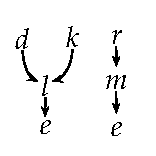
\includegraphics{assets/causal_g.pdf}
    \caption{Causal graph of logic program (\cref{eq:example-cg}).}
    \label{fig:causal-g}
\end{figure}

The tool \textit{xclingo}\footnote{\url{https://github.com/bramucas/xclingo2}}~\cite{Cabalar_2020} 
enables the visualization of justifications for results produced by the \textit{Clingo} solver. 
It does so by incorporating a \src{trace} that corresponds to the rules of the logic program. 
Providing clear explanations of how the framework reaches specific conclusions helps users identify 
potential errors in the construction of the knowledge base and offers transparency for the final outcome. 
This is especially important in medical contexts, where interpretability and trust are critical.

\section{Results}

Evaluation was conducted using publicly available patient data.\footnote{\url{https://www.kaggle.com/datasets/itachi9604/disease-symptom-description-dataset?select=dataset.csv}}
Each patient's list of symptoms serves as input.  
The knowledge base—comprising ASP rules automatically derived  
from medical literature—infers potential diagnoses.  
A prediction is considered correct when the disease inferred  
by the ASP solver matches the actual diagnosis listed in the dataset.

\begin{table}[h]
    \centering
    \begin{tabular}{lcc}
    \hline
    Diseases & Size of Knowledge Base & Accuracy \\
    \hline
    \hline
    Chicken Pox    &  66  & 95\% \\
    Pneumonia      &  75  & 100\% \\
    Common Cold    &  44  & 100\% \\
    \hline
    \end{tabular}
    \caption{Accuracy of the framework on selected diseases. 
    The size column indicates the number of logical terms in the disease-specific ASP program.}
\end{table}

High accuracy is achieved when the knowledge base includes a sufficiently 
rich set of logical rules. The size of this base, measured as the number 
of ASP terms associated with a disease, correlates with prediction performance.

In addition to accurate predictions, \sys offers explainability 
through integration with \src{xclingo}. 
This tool visualizes the reasoning process behind each diagnosis, 
revealing the logical path from symptoms to conclusion.

\begin{lstlisting}[caption={Excerpt from the explanation tree for the chickenpox diagnosis. The structure illustrates the reasoning path based on symptom associations (slightly modified for clarity).},
    label=lst:chickenpox_explanation]{Name}
    *
    |__ diagnosis(chickenpox)
        |__ has(symptom(itching))
        |__ has(symptom(fatigue))
        |__ has(symptom(lethargy))
            |__ has(symptom(fatigue))
            |__ linked_symptom(fatigue, lethargy)
        |__ has(symptom(high_fever))
            |__ has(symptom(mild_fever))
                |__ has(symptom(loss_of_appetite))
                |__ linked_symptom(loss_of_appetite, mild_fever)
            |__ linked_symptom(mild_fever, high_fever)
        |__ has(symptom(loss_of_appetite))
        |__ has(symptom(mild_fever))
            |__ has(symptom(loss_of_appetite))
            |__ linked_symptom(loss_of_appetite, mild_fever)
        |__ has(symptom(swelled_lymph_nodes))
\end{lstlisting}
    
\Cref{lst:chickenpox_explanation} shows an excerpt from the explanation 
tree generated for a patient diagnosed with \textit{chickenpox}. 
The tree visualizes the reasoning steps performed by the ASP solver to reach this conclusion. 
At the root, \sys infers \texttt{diagnosis(chickenpox)} 
based on the presence of multiple symptoms such as \texttt{itching}, \texttt{fatigue}, \texttt{lethargy}, 
and \texttt{high\_fever}. 
Each symptom is further justified through observed inputs or inferred relationships. 
For example, \texttt{lethargy} is supported by repeated instances of \texttt{fatigue} 
and the known association \texttt{linked\_symptom(fatigue, lethargy)}. 
Similarly, \texttt{high\_fever} is explained via the intermediate symptom \texttt{mild\_fever}, 
which itself is supported by \texttt{loss\_of\_appetite}. 
These explanations demonstrate how \sys combines direct observations 
and transitive symptom relationships encoded in the knowledge base to 
construct a transparent and interpretable diagnostic path.

\section{Conclusion}

This work presents a method for automatic disease prediction 
that encodes medical literature and transforms it into ASP code using an LLM. 
It describes the roles of both LLMs and ASP, emphasizing how each contributes to the overall framework. 
The \sys architecture is outlined, along with implementation details for constructing effective prompts 
and structuring rules within the ASP knowledge base.
The method includes predictions for a set of diseases based on the constructed knowledge bases. 
Results show that this approach achieves high-accuracy predictions and provides interpretable explanations.

Future work includes integrating retrieval-augmented generation (RAG) to improve the factual accuracy 
and reliability of the ASP code, and fine-tuning the LLM on clinical reasoning tasks to enhance rule quality. 
Expanding the approach to cover additional diseases is also a key direction.
\newpage
\bibliographystyle{unsrt}
\bibliography{bib}

\end{document}
